
\documentclass[../../../main.tex]{subfiles}

% \tikzexternalize
\begin{document}

	\resizebox{1\textwidth}{!}{




	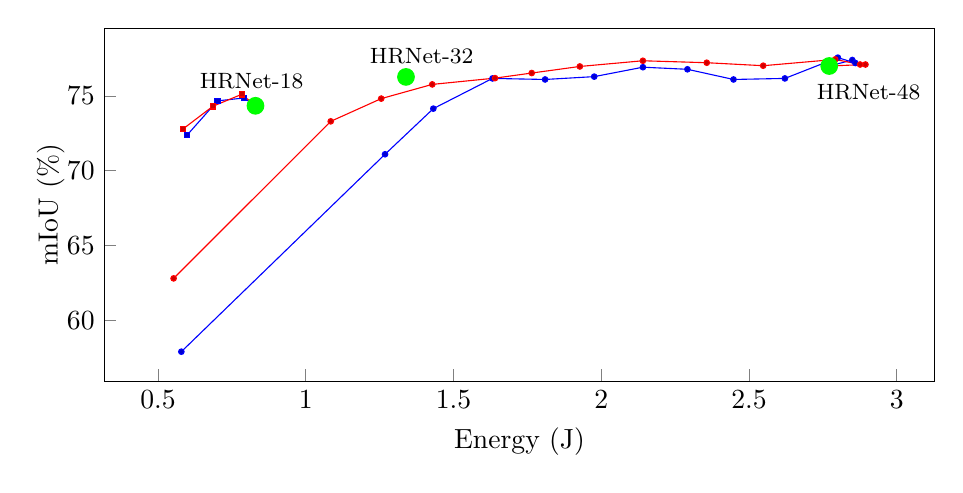
\begin{tikzpicture}
			\begin{axis}[
				ylabel=mIoU (\%),
				% xmode=log,
				% ymin=0,
				% ymax=100,
				mark size = 1pt,
				% xtick={0,2.5,5,7.5,10,12.5,15},
				ytick={60,65,70,75},
				xlabel=Energy (J),
				ylabel shift = -6 pt,
				width=1\textwidth,
				height=0.5\textwidth,
				legend entries={Slimming,  SWD},
				legend to name=sysint_accuracy_legend,
				legend columns=-1,
				legend style = {draw=none},
				xtick pos=left,
                ytick pos=left
				]
				
				\addplot+[mark=*] coordinates 
				{
					
			(2.771487, 77.0)
			(2.849576, 77.4)
			(2.85994, 77.2)
			(2.800701, 77.56)
			(2.621482, 76.17)
			(2.447645, 76.10)
			(2.291658, 76.78)
			(2.141073, 76.92)
			(1.976244, 76.29)
			(1.809942, 76.10)
			(1.63196, 76.17)
			(1.431767, 74.15)
			(1.268395, 71.1)
			(0.579087, 57.9)
					
				% 	%HRNET-18
				% 	(2.619857 , 74.34)
				% 	(1.768388, 74.86)
				% 	(1.587875, 74.67)
				% 	(1.283582, 72.38)
				};
				\addplot+[mark=*] coordinates
				{
					
			(2.771487, 77.0)
			(2.894104, 77.1)
			(2.876006, 77.1)
			(2.791686, 77.44)
			(2.548079, 77.02)
			(2.357087, 77.22)
			(2.14092, 77.35)
			(1.927579, 76.97)
			(1.76483, 76.53)
			(1.640623, 76.19)
			(1.428109, 75.77)
			(1.255498, 74.82)
			(1.084564, 73.3)
			(0.552862, 62.8)
					
					
				% 	%HRNET18
				% 	(2.619857 , 74.34)
				% 	(1.776258, 75.11)
				% 	(1.552426, 74.31)
				% 	(1.246706, 72.79)
				};
				
                \pgfplotsset{cycle list shift=-2}
				\addplot+[mark=square*] coordinates 
				{%HRNET-18
				
					(0.829931 , 74.34)
					(0.790468, 74.86)
					(0.70118, 74.67)
					(0.59846, 72.38)
					
				};
				
				\addplot+[mark=square*] coordinates
				{
				 
					
					%HRNET18
					(0.829931 , 74.34)
					(0.783761, 75.11)
					(0.685882, 74.31)
					(0.584667, 72.79)
				};
				
				\addplot[only marks,
				mark=*,
				mark size=3pt,
				green,
                nodes near coords = HRNet-32,
                nodes near coords align={vertical},
                point meta=y,
                every node near coord/.append style={font=\footnotesize, yshift=0.5mm, xshift=+2mm, color=black},
                ] coordinates
				{
				% 	(5.985977 , 76.27) %baseline Hrnet32
					(1.339235 , 76.27)
				};
				
				\addplot[
				only marks,
				mark=*,
				mark size=3pt,
				green,
                nodes near coords = HRNet-18,
                nodes near coords align={vertical},
                point meta=y,
                every node near coord/.append style={font=\footnotesize, yshift=1mm, xshift=-0.5mm, color=black},
                ] coordinates
				{
				% 	(2.619857 , 74.34) %baseline Hrnet18
					(0.829931 , 74.34)
				};
				
				\addplot[
				only marks,
				mark=*,
				mark size=3pt,
				green,
                nodes near coords = HRNet-48,
                nodes near coords align={vertical},
                point meta=y,
                every node near coord/.append style={font=\footnotesize, yshift=-5.5mm, xshift=5mm, color=black},
                ] coordinates
				{
				% 	(12.147969 , 77) %baseline Hrnet48
					(2.771487, 77.0)
				};
				
				
			\end{axis}
	\end{tikzpicture}
	}
	
	
		\resizebox{1\textwidth}{!}{

	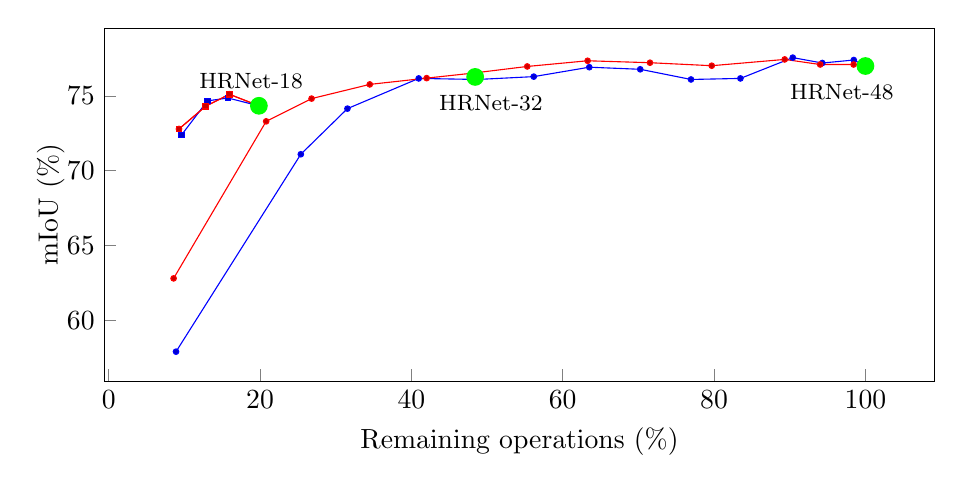
\begin{tikzpicture}
			\begin{axis}[
				ylabel=mIoU (\%),
				% xmode=log,
				% ymin=0,
				% ymax=100,
				mark size = 1pt,
				xtick={0,20,40,60,80, 100},
				ytick={60,65,70,75},
				xlabel=Remaining operations (\%),
				ylabel shift = -6 pt,
				width=1\textwidth,
				height=0.5\textwidth,
				xtick pos=left,
                ytick pos=left
				]
				
				\addplot+[mark=*] coordinates
				{
				    (100 , 77.0) %baseline
				    (98.46, 77.4)
				    (94.3, 77.2)
					(90.4, 77.56) % 10
					(83.48, 76.17) %20
					(76.95, 76.10) %30
					(70.24, 76.78) %40
					(63.51, 76.92) %50
					(56.17, 76.29) %60
					(48.75, 76.10) %70
					(40.97, 76.17) %80
					(31.55, 74.15) %90
					(25.39, 71.1)
					(8.9, 57.9)
					
				% 	%HRNET-18
				% 	(19.85 , 74.34)
				% 	(15.75, 74.86)
				% 	(13.06, 74.67)
				% 	(9.61, 72.38)
				};
				\addplot+[mark=*] coordinates
				{
					(100 , 77.0) %baseline
					(98.44, 77.1)
					(94.02, 77.1)
					(89.33, 77.44)
					(79.69, 77.02)
					(71.53, 77.22)
					(63.29, 77.35)
					(55.31, 76.97)
					(48.23, 76.53)
					(42.02, 76.19)
					(34.5, 75.77)
					(26.81, 74.82)
					(20.81, 73.3)
					(8.58, 62.8)
					
					(19.85 , 74.34)
					(15.95, 75.11)
					(12.82, 74.31)
					(9.29, 72.79)
				};
                \pgfplotsset{cycle list shift=-2}
				\addplot+[mark=square*] coordinates
				{
					%HRNET-18
					(19.85 , 74.34)
					(15.75, 74.86)
					(13.06, 74.67)
					(9.61, 72.38)
				};
				\addplot+[mark=square*] coordinates
				{
					(19.85 , 74.34)
					(15.95, 75.11)
					(12.82, 74.31)
					(9.29, 72.79)
				};
				
				\addplot[only marks,
				mark=*,
				mark size=3pt,
				green,
                nodes near coords = HRNet-32,
                nodes near coords align={vertical},
                point meta=y,
                every node near coord/.append style={font=\footnotesize, yshift=-5.5mm, xshift=2mm, color=black},
                ] coordinates
				{
					(48.43 , 76.27) %baseline Hrnet32
					
				};
				
				\addplot[
				only marks,
				mark=*,
				mark size=3pt,
				green,
                nodes near coords = HRNet-18,
                nodes near coords align={vertical},
                point meta=y,
                every node near coord/.append style={font=\footnotesize, yshift=1mm, xshift=-1mm, color=black},
                ] coordinates
				{
					(19.85 , 74.34) %baseline Hrnet18
					
				};
				
				\addplot[
				only marks,
				mark=*,
				mark size=3pt,
				green,
                nodes near coords = HRNet-48,
                nodes near coords align={vertical},
                point meta=y,
                every node near coord/.append style={font=\footnotesize, yshift=-5.5mm, xshift=-3mm, color=black},
                ] coordinates
				{
					(100 , 77) %baseline Hrnet48
					
				};
				
			\end{axis}
	\end{tikzpicture}



}

	\resizebox{1\textwidth}{!}{

	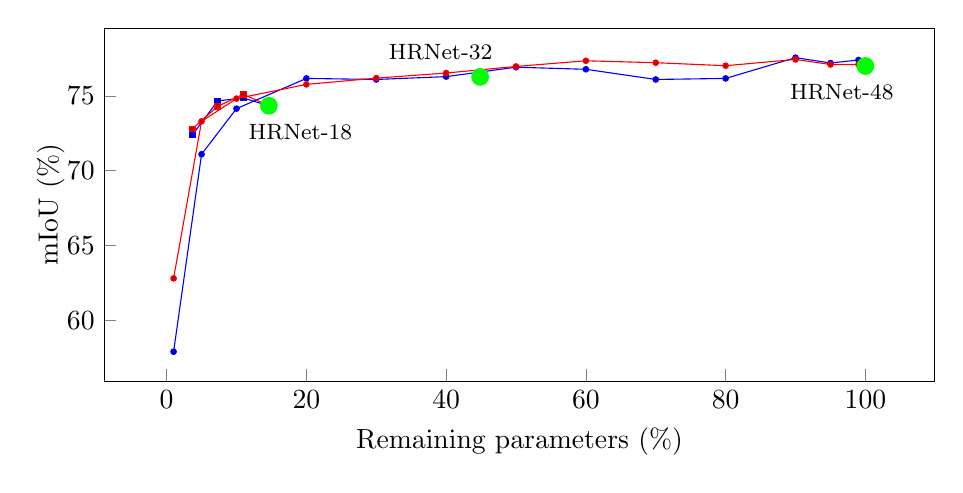
\begin{tikzpicture}
			\begin{axis}[
				ylabel=mIoU (\%),
				% xmode=log,
				% ymin=0,
				% ymax=100,
				mark size = 1pt,
				xtick={0,20,40,60,80, 100},
				ytick={60,65,70,75},
				xlabel=Remaining parameters (\%),
				ylabel shift = -6 pt,
				width=1\textwidth,
				height=0.5\textwidth,
				% legend entries={Slimming, SWD},
				% legend to name=named,
				% legend columns=-1,
				% legend style = {draw=none},
				xtick pos=left,
                ytick pos=left
				]
				
				\addplot+[mark=*] coordinates
				{
				    (100 , 77.0) %baseline
				    (99, 77.4)
				    (95, 77.2)
					(90, 77.56) % 10
					(80, 76.17) %20
					(70, 76.10) %30
					(60, 76.78) %40
					(50, 76.92) %50
					(40, 76.29) %60
					(30, 76.10) %70
					(20, 76.17) %80
					(10, 74.15) %90
					(5, 71.1)
					(1, 57.9)
					
				% 	(14.64 , 74.34)
				% 	(10.98, 74.86)
				% 	(7.32, 74.67)
				% 	(3.66, 72.38)
					
				};
				\addplot+[mark=*] coordinates
				{
					(100 , 77.0) %baseline
					(99, 77.1)
					(95, 77.1)
					(90, 77.44)
					(80, 77.02)
					(70, 77.22)
					(60, 77.35)
					(50, 76.97)
					(40, 76.53)
					(30, 76.19)
					(20, 75.77)
					(10, 74.82)
					(5, 73.3)
					(1, 62.8)
					
				% 	(14.64 , 74.34)
				% 	(10.98, 75.11)
				% 	(7.32, 74.31)
				% 	(3.66, 72.79)
				};
				\pgfplotsset{cycle list shift=-2}
				\addplot+[mark=square*] coordinates
				{
					(14.64 , 74.34)
					(10.98, 74.86)
					(7.32, 74.67)
					(3.66, 72.38)
					
				};
				\addplot+[mark=square*] coordinates
				{
					(14.64 , 74.34)
					(10.98, 75.11)
					(7.32, 74.31)
					(3.66, 72.79)
				};
				
				\addplot[only marks,
				mark=*,
				mark size=3pt,
				green,
                nodes near coords = HRNet-32,
                nodes near coords align={vertical},
                point meta=y,
                every node near coord/.append style={font=\footnotesize, yshift=1mm, xshift=-5mm, color=black},
                ] coordinates
				{
					(44.86 , 76.27) %baseline Hrnet32
					
				};
				
				\addplot[
				only marks,
				mark=*,
				mark size=3pt,
				green,
                nodes near coords = HRNet-18,
                nodes near coords align={vertical},
                point meta=y,
                every node near coord/.append style={font=\footnotesize, yshift=-5.5mm, xshift=4mm, color=black},
                ] coordinates
				{
					(14.64 , 74.34) %baseline Hrnet18
					
				};
				
				\addplot[
				only marks,
				mark=*,
				mark size=3pt,
				green,
                nodes near coords = HRNet-48,
                nodes near coords align={vertical},
                point meta=y,
                every node near coord/.append style={font=\footnotesize, yshift=-5.5mm, xshift=-3mm, color=black},
                ] coordinates
				{
					(100 , 77) %baseline Hrnet48
					
				};
				
			\end{axis}
	\end{tikzpicture}
}
\begin{center}

    \ref*{sysint_accuracy_legend}
\end{center}



\end{document}
